\subsubsection{UC\theuccount-PR - Redmine segnala apertura issue al Producer Redmine}
%    \begin{figure}[H]
%		\centering
%		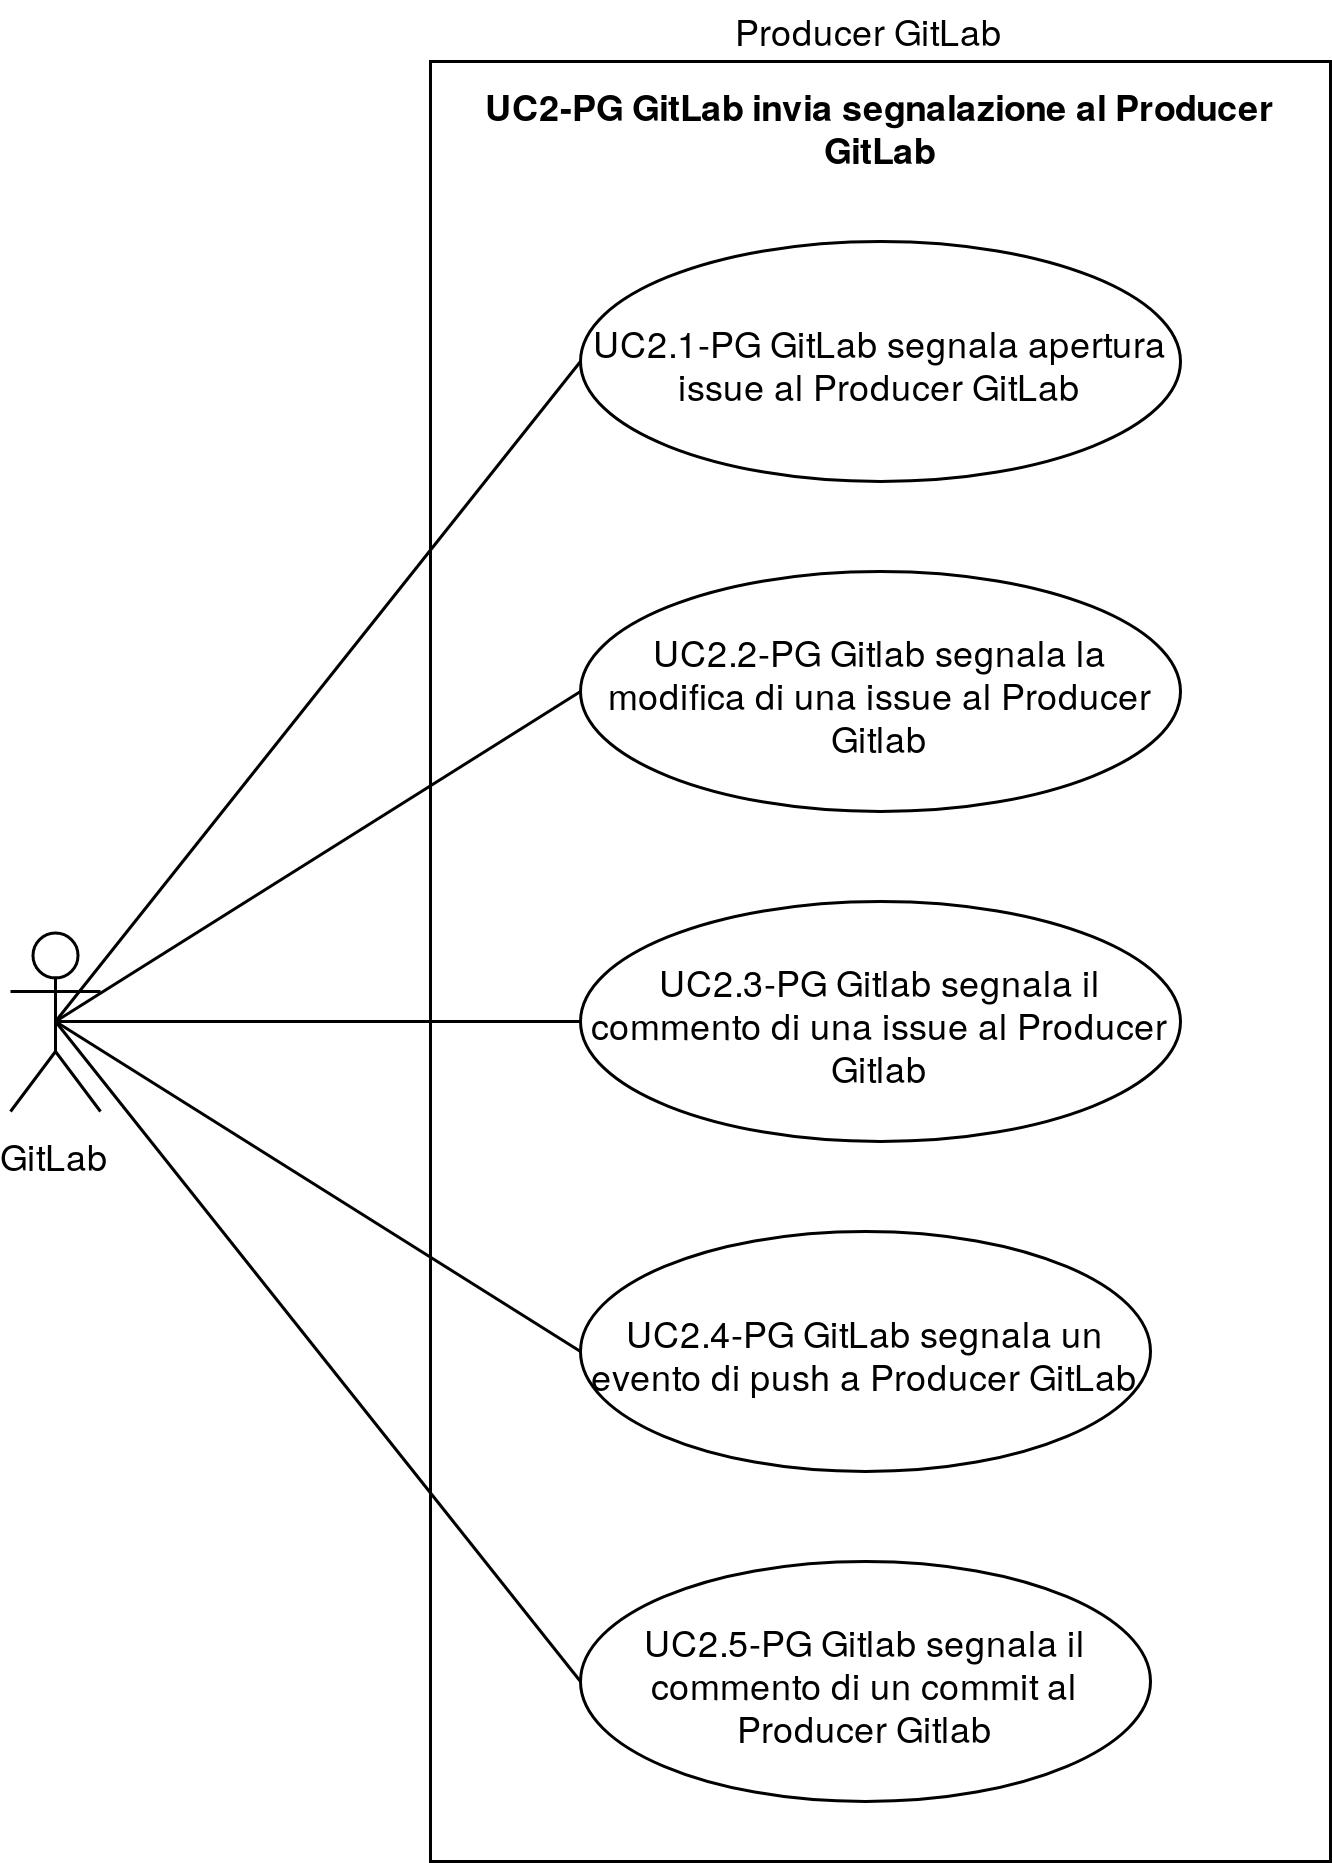
\includegraphics[width=0.5\textwidth]{img/casi_d'uso/UC2.png}\\
%		\caption{UC\theuccount-PR - Redmine segnala apertura issue al Producer Redmine}
%	\end{figure}
	\begin{itemize}
		\item \textbf{Codice}: UC\theuccount-PR.
		\item \textbf{Titolo}: Redmine segnala apertura issue al Producer Redmine.
		\item \textbf{Attori primari}: Redmine.
		\item \textbf{Descrizione}: Redmine segnala a \progetto\ l'apertura di una nuova issue tramite webhook.
		
		L'apertura di una issue in un particolare progetto su Redmine contiene i seguenti campi di interesse:
		 \begin{itemize}
		 	\item Tracker
		 	\item Subject
		 	\item Status
		 	\item Priority e opzionalmente:
		 	\begin{itemize}
		 		\item Description
		 		\item Assignee
		 	\end{itemize}
		 \end{itemize}
		\item \textbf{Precondizione}: Viene aperta una issue su Redmine da
		segnalare a \progetto.
		\item \textbf{Postcondizione}: il Producer Redmine riceve la segnalazione da Redmine.
		\item \textbf{Scenario principale}: 
		\begin{enumerate}
			\item Viene aperta una nuova issue su Redmine
			\item Redmine procede all'invio della segnalazione di issue al Producer Redmine
		\end{enumerate}
		
	\end{itemize}
